





\section{Introduction}



Semantic image segmentation aims to predict a category label for every image pixel,
which is an important yet challenging task for image understanding.
Recent approaches have applied convolutional neural network (CNNs) \cite{farabet2013learning,LongSD14,ChenPKMY14}
to this pixel-level labeling task and achieved remarkable success.
Among these CNN-based methods, fully convolutional neural networks (FCNNs)~\cite{LongSD14,ChenPKMY14}
have become a popular choice, because of their computational efficiency for dense prediction and end-to-end style learning.




Contextual relationships are ubiquitous and provide important cues for scene understanding tasks.
Spatial context can be formulated in terms of  semantic compatibility relations between one object and its neighboring objects or image patches (stuff), in which a compatibility relation is an indication of the co-occurrence of visual patterns.
For example, a car is likely to appear over a road, and a glass is likely to appear over a table.
Context can also encode incompatibility relations.
For example, a car is not likely to be surrounded by sky.  These relations also exist
at finer scales, for example, in
object part-to-part relations, and part-to-object relations.
In some cases, contextual information is the most important cue, particularly when a single object shows significant visual ambiguities.
A more detailed discussion of the value of spatial context can be found in \cite{heitz2008learning}.






\begin{figure}[t]
	\centering
	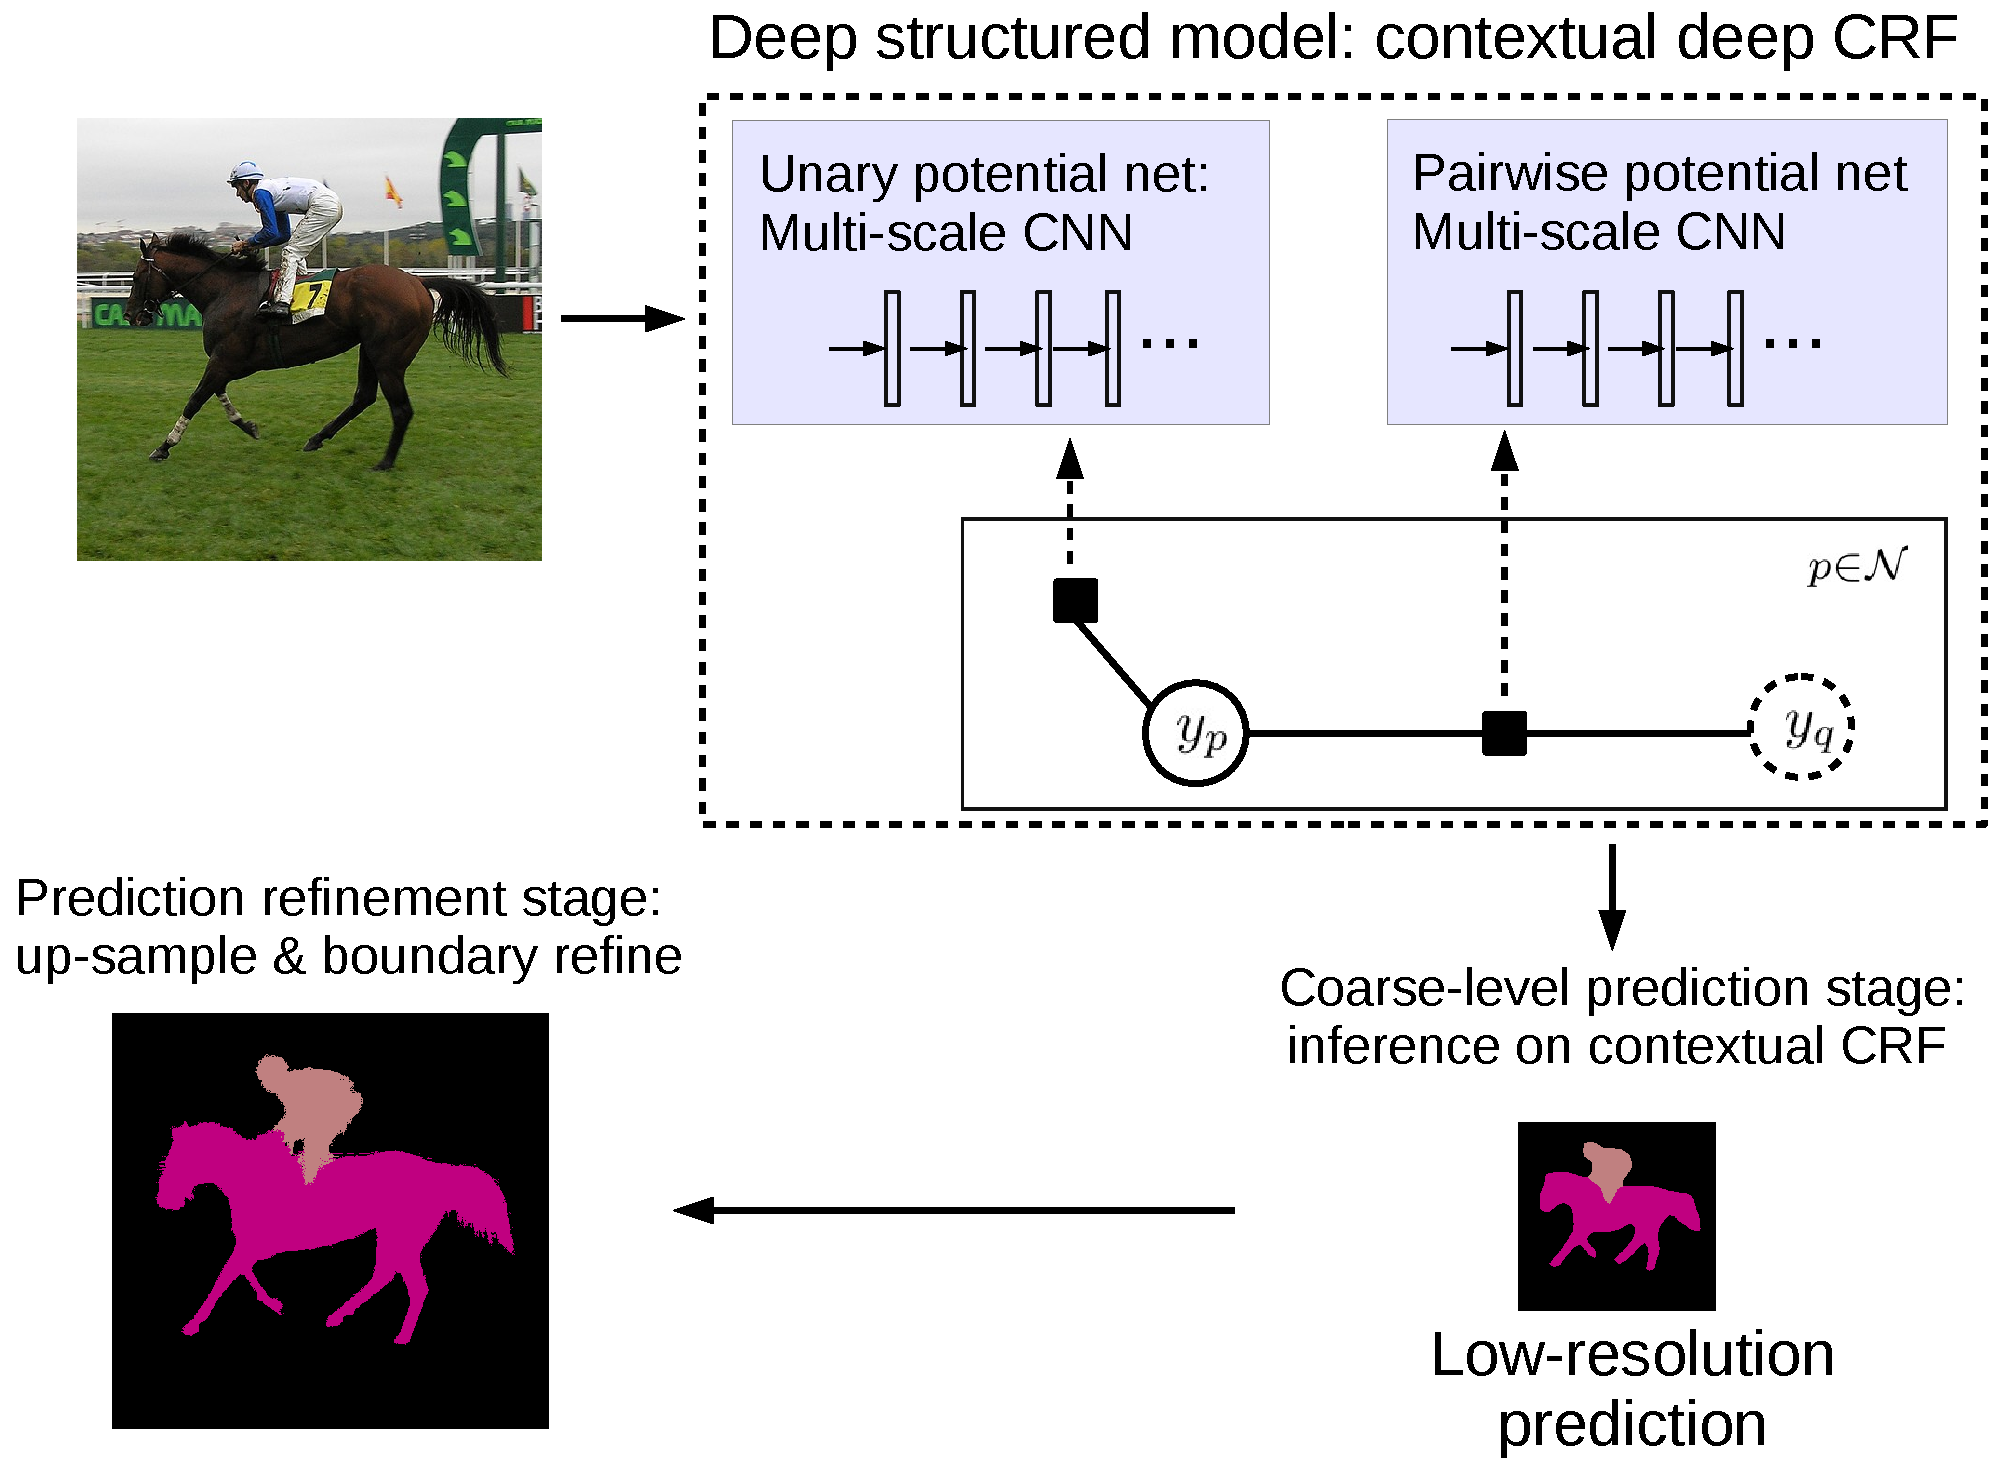
\includegraphics[width=.95\linewidth]{./figs/general_graph}
\caption{An illustration of the prediction process of our method.
Both our unary and pairwise potentials are formulated as multi-scale CNNs for capturing semantic relations between image regions.
Our method outputs low-resolution prediction after CRF inference, then the prediction is up-sampled and refined in a standard post-processing stage to output the final prediction.}
\label{fig:general_graph}
\end{figure}




We explore two types of spatial context to improve the segmentation performance: patch-patch context and patch-background context.
The patch-patch context is the semantic relation between the visual patterns of two image patches. Likewise,
patch-background context is the semantic relation between a patch and a large background region.




Explicitly modeling the patch-patch contextual relations has not been well studied in recent CNN-based segmentation methods.
In this work, we propose to explicitly model the contextual relations using conditional random fields (CRFs).
We formulate CNN-based pairwise potential functions to capture semantic correlations between neighboring patches.
Some recent methods  combine CNNs and CRFs for semantic segmentation,
e.g., the dense CRFs applied in \cite{ChenPKMY14,schwing2015fully,zheng2015conditional,Dai2015arXiv}.
The purpose of applying the dense CRFs in these methods is to refine the upsampled low-resolution prediction to sharpen object/region boundaries.
These methods consider Potts-model-based pairwise potentials for enforcing local smoothness.
There the pairwise potentials are conventional log-linear functions.
In contrast, we
learn more general pairwise potentials using CNNs to model the semantic compatibility between image regions.
Our CNN pairwise potentials aim to improve the coarse-level prediction rather than doing local smoothness, 
and thus have a different purpose compared to Potts-model-based pairwise potentials.
Since these two types of potentials have different effects, they can be combined to improve the segmentation system.
Fig.~\ref{fig:general_graph} illustrates our prediction process.




In contrast to patch-patch context,
patch-background context is widely explored in the literature.
For CNN-based methods,
background information can be effectively captured
by combining features from a multi-scale image network input, and has shown good performance
in some recent segmentation methods \cite{farabet2013learning,MostajabiYS14}.
A special case of capturing patch-background context is considering the whole image as the background region and incorporating the image-level label information into learning.
In our approach, to encode rich background information, we construct multi-scale networks and apply sliding pyramid pooling on feature maps.
The traditional pyramid pooling (in a sliding manner) on the feature map is able to capture information from background regions of different sizes.



Incorporating general pairwise (or high-order) potentials usually involves expensive inference, which brings challenges for CRF learning.
To facilitate efficient learning we apply piecewise training of the CRF \cite{SuttonM05} to avoid repeated inference
 during back propagation training.





Thus our main \emph{contributions} are as follows.

  { 1.}~We formulate CNN-based general pairwise potential functions in CRFs to explicitly model patch-patch semantic relations.


  { 2.}~Deep CNN-based general pairwise potentials are challenging for efficient CNN-CRF joint learning.
  We perform approximate training, using piecewise training of CRFs \cite{SuttonM05}, 
  to avoid the repeated inference at every stochastic gradient descent iteration and thus achieve efficient learning.


  {3.}~We explore background context by applying a network architecture with traditional multi-scale image input \cite{farabet2013learning} 
  and sliding pyramid pooling \cite{lazebnik2006beyond}.
   We empirically demonstrate the effectiveness of this network architecture for semantic segmentation.


  {4.}~We set new state-of-the-art performance on a number of popular semantic segmentation datasets, including NYUDv2, PASCAL VOC 2012, PASCAL-Context, and SIFT-flow.
	In particular, we achieve an intersection-over-union score of $78.0$ on the PASCAL VOC 2012 dataset, which is {\em  the  best reported result} to date.






\subsection{Related work}

Exploiting contextual information
has been widely studied in the literature (e.g., \cite{rabinovich2007objects,heitz2008learning,doersch2014context}).  
For example, the early work ``TAS'' \cite{heitz2008learning} models different types of spatial context between {\em Things} and {\em Stuff}
using a generative probabilistic graphical model.


The most successful recent methods for semantic image segmentation are based on CNNs.
A number of these CNN-based methods for segmentation are region-proposal-based methods \cite{GirshickDDM13,BharathECCV2014}, which first generate region proposals and then assign category labels to each.  Very recently,  FCNNs
 \cite{LongSD14,ChenPKMY14,Dai2015arXiv} have become a popular choice for semantic segmentation, because of their effective feature generation and end-to-end training.
FCNNs
have also been applied to a range of other dense-prediction tasks recently,
 such as image restoration \cite{Eigen_iccv13}, image super-resolution \cite{Dong_eccv14}
 and depth estimation \cite{dcnn_nips14,liu2014deep}.
The method we propose here is similarly
built upon fully convolution-style networks.


The direct prediction of FCNN based methods usually are in low-resolution.
To obtain high-resolution predictions, a number of recent methods focus on refining the low-resolution prediction to obtain high resolution prediction.
DeepLab-CRF \cite{ChenPKMY14} performs bilinear upsampling of the prediction score map to the input image size and apply the dense CRF method \cite{krahenbuhl2012efficient} to refine the object boundary by leveraging the color contrast information.
CRF-RNN \cite{zheng2015conditional} extends this approach by implementing recurrent layers for end-to-end learning of the dense CRF and the FCNN network.
The work in \cite{noh2015learning} learns deconvolution layers to upsample the low-resolution predictions.
The depth estimation method \cite{liu2015learning} explores super-pixel pooling 
for building the gap between low-resolution feature map and high-resolution final prediction.
Eigen \textit{et~al.} \cite{eigen2015predicting} perform coarse-to-fine learning of multiple networks with different resolution outputs for refining the coarse prediction.
The methods in \cite{hariharan2014hypercolumns,LongSD14} explore middle layer features (skip connections) for high-resolution prediction.
Unlike these methods, our method focuses on improving the coarse (low-resolution) prediction 
by learning general CNN pairwise potentials to capture semantic relations between patches.
These refinement methods are complementary to our method.



Combining the strengths of CNNs and CRFs for segmentation
has been the focus of several recently developed approaches.
DeepLab-CRF in \cite{ChenPKMY14} trains FCNNs and applies a dense CRF~\cite{krahenbuhl2012efficient} method
as a post-processing step.
CRF-RNN \cite{zheng2015conditional} and the method in \cite{schwing2015fully} extend DeepLab and \cite{krahenbuhl2013parameter} by jointly learning the dense CRFs and CNNs.  They consider Potts-model based  pairwise potential functions which  enforce smoothness only.
The CRF model in these methods is for refining the up-sampled prediction.
Unlike  these methods, our approach learns CNN-based pairwise potential functions for modeling semantic relations between patches.



Jointly learning CNNs and CRFs has also been explored in other applications apart from segmentation.
The recent work in \cite{liu2014deep,liu2015learning} proposes to jointly learn {\em continuous} CRFs and CNNs for depth estimation
from  single monocular images. 
The work in \cite{Lecun_nips14} combines CRFs and CNNs for human pose estimation.
The authors of \cite{chen2014learning} explore joint training of Markov random fields and deep neural networks for predicting words from noisy images and image s classification. Different from these methods, we explore efficient piecewise training of CRFs with CNN pairwise potentials.


